\documentclass{article}

\usepackage[affil-it]{authblk}

\usepackage[USenglish,american]{babel}

\usepackage{amsfonts,amsmath,amsthm,amssymb}

\usepackage{tikz}
\usepackage{float}
\setlength{\parindent}{0mm}
\setlength{\parskip}{.5em}
\usepackage[letterpaper, margin=1in]{geometry}
%\usepackage{showframe}
\usepackage{graphicx}

\usepackage{multicol,caption}
\setlength\columnsep{25pt}

\usepackage{enumerate}

\usepackage{verbatim}
\usepackage{listings}

\usepackage{siunitx}

\usepackage{color}

%%
%% Julia definition (c) 2014 Jubobs
%%
\lstdefinelanguage{Julia}%
  {morekeywords={abstract,break,case,catch,const,continue,do,else,elseif,%
      end,export,false,for,function,immutable,import,importall,if,in,%
      macro,module,otherwise,quote,return,switch,true,try,type,typealias,%
      using,while},%
   sensitive=true,%
   alsoother={$},%
   morecomment=[l]\#,%
   morecomment=[n]{\#=}{=\#},%
   morestring=[s]{"}{"},%
   morestring=[m]{'}{'},%
}[keywords,comments,strings]%

\lstset{%
    language         = Python,
    basicstyle       = \footnotesize\ttfamily,,
    keywordstyle     = \bfseries\color{blue},
    stringstyle      = \color{magenta},
    commentstyle     = \color{red},
    showstringspaces = false,
    backgroundcolor  = \color{lightgray},
    numbers          = left,
    title            = \lstname,
    numberstyle      = \tiny\color{lightgray}\ttfamily,
}

\usepackage{xspace}
\usepackage{url}
\usepackage{cite}

\usepackage{coffee4}

\newcommand{\Bold}{\mathbf}


\title{Denoising and Labeling Hydrophone Data}
\date{\today}
\author{Philip Robinson}
\affil{Oregon Health Sciences University}

\begin{document}


\maketitle


\begin{abstract}
  There is a need for an index of acoustic events and associated metadata for University of Hawaii's Aloha Cabled Observatory (ACO) hydrophone recordings. Currently searching the audio recordings is done at human pace by listening to the audio stream, which is prohibitive at approximately 10 years of content.
The proposal is to develop a processing system that creates simple data store of vocals and metadata associated with vocalization events, renders a denoised~\cite{Baskar2015StudyOD,specsub2008,Berouti1979EnhancementOS} copy of those vocalization events, and provide a simple time based retrieval system. The system is written using \texttt{python} and the \texttt{scipy}~\cite{Jones2001} libraries for signal processing. %
 The extended goal of this work is to use whale vocalization as a proxy measurement of migration patterns, and attempt to identify migratory changes against known climate events. In order to accomplish this task, noise in audio recording should be smoothed or removed, vocalizations must be localized/indexed, features of speech must be extracted, species must be identified~\cite{2014ASAJ} or clustered.
% , \texttt{ponyorm} for light weight authoring of data store, and \texttt{paramiko} if needed for accessing remote recordings of original data.
\end{abstract}

\begin{multicols}{2}

\section{Introduction}

University of Hawaii's ACO has approximately 10 years of hydrophone data, in need of indexing, labeling, and cleaning. To enable further research and bootstrap more advanced indexing techniques, a data retrieval, analysis, and labeling tool is Provided is a simple module enabling these three features. The module provided include:

\begin{itemize}
    \setlength\itemsep{0em}
\item reading \& listen to ACO encoded data
\item standard \texttt{datetime} units for navigation
\item parameterized visualizations for audio units
\item simple denoising via spectral subtraction
\item center wave by empirical mode decomposition
\end{itemize}

\section{Data Retrieval}

The ACO data is gathered at N$22^\circ45.110'$ W$158^\circ00'$.
The recordings are encoded as variable bit-width raw sensor readings (fixed-width for each chunk of 4096 samples). Each file is saved as a 5 minute chunk, named with it's datetime stamp. The set elected for this project was 24K samples per second (there exists a 96K as well).


\begin{figure}[H]
  \centering

\begin{lstlisting}
from aco import ACOio, datetime, timedelta

loader = ACOio('./basedir/')
target = datetime(
    day=18, month=2, year=2016,
    hour=7, minute=55
)

src = loader.load(datetime)
snip = src[
  timedelta(seconds=7):
  timedelta(seconds=11)
]
snip.View()
\end{lstlisting}

  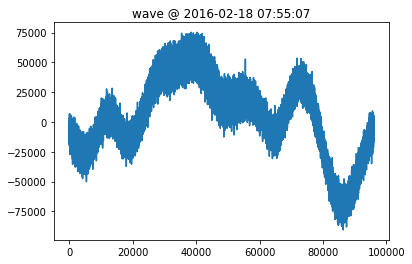
\includegraphics[width=\columnwidth]{./rawwave.png}
  \caption{Raw Data}
  \label{fig:rawwav}

\end{figure}

It is visible, from \texttt{(Figure~\ref{fig:rawwav})} that the direct current gain is not centered at zero, nor trivially accumulative. This is a consequence of changes in atmospheric pressure, due to the ocean's motion, attenuating the signal. Without these changes in atmospheric pressure the current gain can be corrected by removing the mean of the original signal, however in this case empirical mode decomposition is used to yield more accurate results. This will be addressed in greater detail later.

\begin{figure}[H]
  \centering

  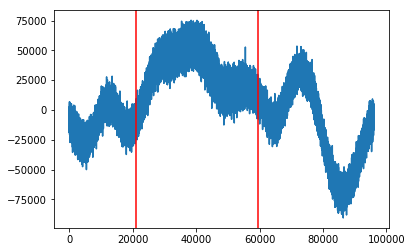
\includegraphics[width=\columnwidth]{./rawvocal.png}
  \caption{Raw Vocalization}
  \label{fig:rawvoc}

\end{figure}

It is also not obvious this track has a vocalization, highlighted in \texttt{(Figure~\ref{fig:rawvoc})}. This pattern is indicative of high amounts of noise. Usually, a better perspective is gained using the \texttt{logspectrum}, however as seen \texttt{(Figure~\ref{fig:rawspec})} this is mostly non-informative. This is for two reasons. Firstly, the dynamic range of the track is too great due to the direct current gain as mentioned above. Secondly, the sampling rate is too high, resulting in far too much data being expressed in a small amount of space, which this expensive run-time effects on complicated processing algorithms, like empirical mode decomposition.

\begin{figure}[H]
  \centering
\begin{lstlisting}
snip.View(
  'logspectrum',
  frame_duration=.08,
  frame_shift=.02
)

\end{lstlisting}
  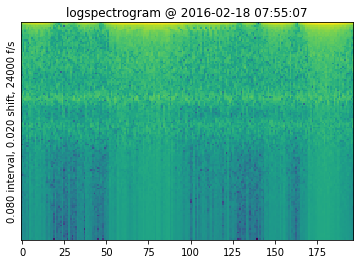
\includegraphics[width=\columnwidth]{./rawspec.png}
  \caption{Raw Spectrogram}
  \label{fig:rawspec}

\end{figure}

\section{Spectral Subtraction}

Spectral subtraction is a technique used to denoise signals with additive white noise (like found in this application). It is also, a very cheap algorithm with many modifications~\cite{specsub2008}, which makes it an ideal first pass on the data.

The sampled signal $y$ is modeled as the desired signal $x$ and background noise $b$. \[y[n] = x[n] + b[n]\]
At a single frame at point $p$ and length $L$,
\begin{align*}
  Y(pL, \omega) &= X(pL, \omega) + B(pL, \omega)\\
  |Y(pL, \omega)|^2 &= |X(pL, \omega)|^2 \\&+|B(pL, \omega)|^2 + |X(pL, \omega)*B(pL, \omega)|\\
\end{align*}

We can estimate the background noise, given sufficiently small frames, by subtracting the mean power spectrum from a segment of only noise. Using Welch's method~\cite{welch1976} we are able to estimate the mean power spectrum.

\begin{figure}[H]

\begin{lstlisting}
def _spectral_subtraction(self, other,
    frame_duration=.08, frame_shift=.02,
    wtype='boxcar', alpha=5.0, beta=.01):

  Frames = self._Frame(
    frame_duration, frame_shift).data
  power = other.power(
    frame_duration, frame_shift, wtype)
  window = signal.get_window(
    wtype, self.to_frame_count(frame_duration))

  spectrum = np.fft.fft(Frames * window)
  amplitude = np.abs(spectrum)
  phase = np.angle(spectrum)

  _ = (amplitude ** 2.0) - (power * alpha)
  _ = np.maximum(_, beta * amplitude ** 2.0)
  _ = np.sqrt(_)
  _ = _ * np.exp(phase*1j)

  return _
\end{lstlisting}
  \caption{Spectral Subtraction}
  \label{fig:subtractpy}

\end{figure}

Rather than the original spectral subtraction algorithm, \texttt{(Figure~\ref{fig:subtractpy})} implements the algorithm found in ~\cite{Berouti1979EnhancementOS}. This allows for adjustable $\alpha$ and $\beta$ parameters, used in tuning some audio artifacts consequent of spectral subtraction.

From \texttt{(Figure~\ref{fig:subtract})} it is much easier to see the vocalization section in the waveform. It is apparent that the spectrogram has less noise, but not necessarily in a useful way. This is due to the dynamic range and resolution problems mentioned above.


\begin{figure}[H]
  \centering

  \begin{comment}
\begin{lstlisting}
noise = snip[
  timedelta(seconds=0):
  timedelta(seconds=.8)]
clean = snip.subtract(noise)
clean.View()
clean.View('logspectrogram')
\end{lstlisting}
\end{comment}

  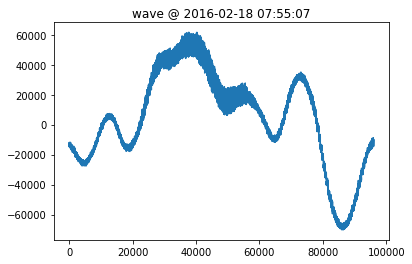
\includegraphics[width=\columnwidth]{./subwave.png}
  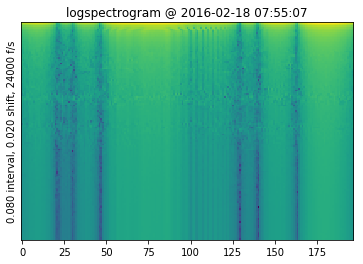
\includegraphics[width=\columnwidth]{./subspec.png}

  \caption{After Subtraction}
  \label{fig:subtract}

\end{figure}

\begin{figure}[H]
  \centering
  \begin{lstlisting}
noise = snip[
  timedelta(seconds=0):
  timedelta(seconds=.8)
]
clean = snip.subtract(noise)
down = clean.resample(40000)
down.View(
  'logspectrum',
  frame_duration=.08,
  frame_shift=.02
)
\end{lstlisting}
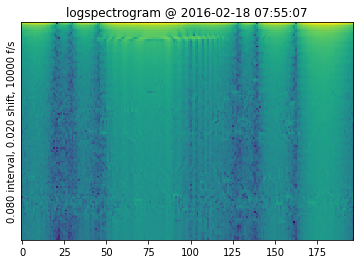
\includegraphics[width=\columnwidth]{./downspec.png}
  \caption{After Resamling}
  \label{fig:resample}

\end{figure}

Down sampling the data, as shown \texttt{(Figure~\ref{fig:resample})}, gives us the first visible pattern in the spectrogram. It is faint, due to far too high of dynamic range in the waveform.


\section{Empirical Mode Decomposition}

Empirical Mode Decomposition is used to address the variable gain found in this waveform, and allow us a more informative exploratory data analysis. Empirical mode decomposition expresses the current waveform as a summation of sine functions of learned mode. The results are stored, ordered by highest to lowest frequency. We can sum the first $k$ levels of the yield to capture the majority of data and audible effects, while ignoring the low order functions (that encode the gain).

This is a computationally expensive procedure, that benefits from the down sampling step.

\begin{figure}[H]
  \centering
  \begin{lstlisting}
centered = down.remove_dc(levels=13)
centered.View()
centered.View(
  'logspectrum',
  frame_duration=.08,
  frame_shift=.02
)
\end{lstlisting}
  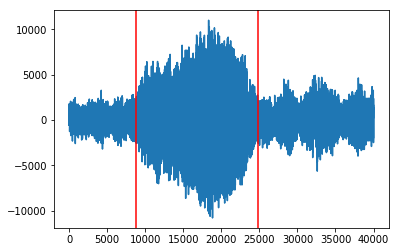
\includegraphics[width=\columnwidth]{./centered.png}
  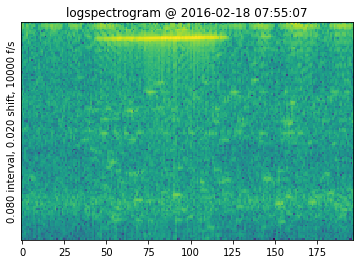
\includegraphics[width=\columnwidth]{./centeredspec.png}
  \caption{After EMD}
  \label{fig:emd}

\end{figure}

\section{Labeling}

With this level of granularity, we can correctly label our original dataset using both auditory and visual queues.

\begin{figure}[H]
  \centering
  \begin{lstlisting}
noise.label_src_as_noise()
centered[
  timedelta(seconds=0.88):
  timedelta(seconds=2.48)
].label_src_as_voice()
\end{lstlisting}

  \caption{Label Sections of Audio}
  \label{fig:labeling}
\end{figure}


\section{Results}

With the right parameters, this works very well to clean the data visually and audibly. Unfortunately, not all theses parameters have obvious or predictable trends. The goal of being able to with high precision label vocalization for later learned methods is definitely hit, and the ability to encode metadata enabling better audio track retrieval for human perception is on its way.

\begin{comment}
\section{Prior Work}
\section{Methods}
\section{Materials}
\section{Results}
\section{Discussion}
\subsection{Study Assumptions}
\end{comment}
\bibliography{references.bib}{}
\bibliographystyle{plain}



\end{multicols}

\end{document}
